\setchapterpreamble[u]{\margintoc}
\chapter{Process Management}
\labch{procman}

\section{What is sleep?}

\texttt{sleep} is a command that is used to delay the execution of a process
for a specified amount of time. \textbf{sleep} itself is a no-op command,
\footnote{
  NO-OP stands for No Operation. It is a command that does nothing.
  More reading on NO-OP can be found
  \href{https://en.wikipedia.org/wiki/NOP\_(code)}{here}.
}
but it takes a variable amount of time to execute, depending on the argument
of the command. This is useful when you want to delay the execution of another
command or chain of commands by a certain amount of time.

\subsection{Example}

\begin{lstlisting}[language=bash]
$ sleep 5
$ echo "Hello, World!"
Hello, World!
\end{lstlisting}

\subsection{Scripting with sleep}

If you run the above snippet, you will see that the output is delayed by 5 seconds.
Moreover, the prompt itself will not be available for 5 seconds, as the shell is busy
with executing the \texttt{sleep} command.
To run the entire snippet as one process, simply put the two commands on
separate lines of a file (say, \texttt{hello.sh}), and run the file as a script.

\begin{lstlisting}[language=bash]
$ cat hello.sh
sleep 5
echo "Hello, World!"
$ bash hello.sh
Hello, World!
\end{lstlisting}

We will be using \texttt{sleep} in the examples throughout this chapter to demonstrate
process management since it is a simple command that can be used to quickly
spawn an idempotent process for any arbitrary amount of time.

\subsection{Syntax and Synopsis}

\begin{lstlisting}[language=bash]
sleep NUMBER[SUFFIX]...
\end{lstlisting}

Here the \texttt{NUMBER} is the amount of time to sleep.
The \texttt{SUFFIX} can be \texttt{s} for seconds, \texttt{m} for minutes,
\texttt{h} for hours, and \texttt{d} for days.

\section{Different ways of running a process}

\subsection{What are processes?}

\begin{definition}[Process]
  A process is an instance of a program that is being executed.
  It contains the program code and its current activity.
  Depending on the operating system (OS), a process may be made up of
  multiple threads of execution that execute instructions concurrently.
  Several processes may be associated with the same program; for example,
  opening up several instances of the same program often means more than
  one process is being executed.
  Each process has its own `process id` or \textbf{PID} to uniquely identify it.
\end{definition}

Whenever we run an application, or even a command on the linux shell, it spawns a process. Processes are always created by an already
existing process
\sidenote{
  Other than the very first process, which is always the
  \textbf{init} process. In most distributions, this is
  done by
  \href{https://systemd.io/}{systemd}, which is an
  init system that does a lot of other things as well.
  You can learn more about systemd and what all
  it does
  \href{https://documentation.suse.com/external-tree/en-us/sles/12-SP4/systemd\_in\_suse\_linux\_enterprise\_12\_white\_paper.pdf}{here}.
}
This creates a tree-like structure of processes, where each process has a parent process and can have multiple child processes.
When the parent of a process dies, the child processes are adopted by the \textbf{init} process.
\textbf{init} is thus the root of the process tree.

\begin{figure}[h!]
  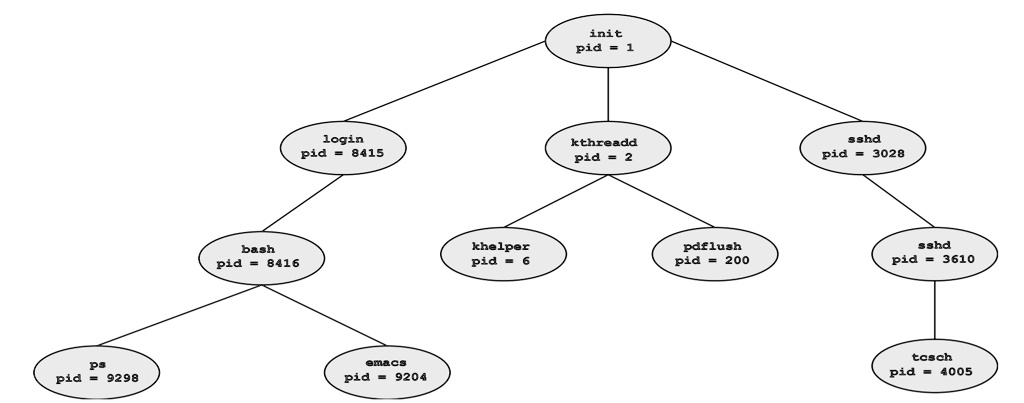
\includegraphics{process-tree}
  \caption{Example of a process tree}
  \labfig{process-tree}
\end{figure}

\subsection{Process Creation}
In linux systems, processes are managed by the kernel.
The kernel is responsible for creating, scheduling, and destroying processes.
The user can interact with the kernel using system calls to create, manage, and destroy processes.
Creating processes is simple, and can be done using the \textbf{fork()} system call.
This is used when any process wants to create a new process.

To simply create a new process for a command,
we can simply type in the command and press enter.
This will not only fork a new process from the terminal or
terminal emulator as the parent process, but also tie the
standard input, standard output, and standard error of the child process
to the terminal or terminal emulator.
\sidenote{
  Standard Input, Output, and Error are the default streams that are used by
  the shell to interact with the user. Standard Input is used to take input from
  the user, Standard Output is used to display output to the user, and Standard Error
  is used to display errors to the user. We will cover these in details in the next chapter.
}

\begin{lstlisting}[language=bash]
$ sleep 5
\end{lstlisting}

This will create a new process that will sleep for 5 seconds.

Remember that each process has a unique process id (PID).
Each process also has a parent process id (PPID),
which is the PID of the parent process.
If a process is created by the shell, the shell will be the parent process.
If the shell's process is killed, the child process will also
be killed, as the child process is owned by the shell.

\subsection{Process Ownership}

If you are using a linux operating system with a GUI server (X or Wayland),
try the following to understand how process ownership works.

Open two terminals, in the first one, run \texttt{echo \$\$} to see the
process ID of that shell.
It should print out a random string of digits, that is the PID of the shell.
Then run a GUI application, such as \textbf{firefox}.
\sidenote{
  Make sure you are running something that is not running already.
}
This will block your terminal and open a new window of firefox.

\begin{lstlisting}[language=bash]
$ echo $$
2277503
$ firefox
\end{lstlisting}

Now in the other terminal, which is free, run \texttt{pgrep firefox}
\sidenote{
  or whatever was your process's name
}
It should print out another random string of digits, it is the PID of
firefox.

Now you can use the following command to find the parent process's process
ID (PPID) to verify it is the same as the output of \texttt{\$\$} in the first terminal.

\begin{lstlisting}[language=bash]
$ pgrep firefox
2278276
$ ps -efj | awk '$2==2278276;NR==1'
UID          PID    PPID    PGID     SID  C STIME TTY          TIME CMD
sayan    2278276 2277503 2278276 2277503 12 16:59 pts/5    00:00:03 /usr/lib/firefox/firefox
\end{lstlisting}

Here we can see that the PPID of firefox is the PID of the shell.

Note that the second command should put the PID of firefox, which we got
from the previous command. This can also be done in a single command
which you can directly copy and paste in your terminal.

\begin{lstlisting}[language=bash]
$ ps -efj | awk "\$2==$(pgrep firefox);NR==1"
UID          PID    PPID    PGID     SID  C STIME TTY          TIME CMD
sayan    2278276 2277503 2278276 2277503  1 16:59 pts/5    00:00:04 /usr/lib/firefox/firefox
\end{lstlisting}

Now, what happens if we kill the parent process?
To kill a process all we need to use is use the \texttt{kill}
command with the PID of the process.

\begin{lstlisting}[language=bash]
$ kill -9 2277503
\end{lstlisting}

\marginnote{
  The \texttt{-9} flag is used to send a \textbf{SIGKILL} signal to the process.
  This signal is used to kill a process immediately.
  We will cover signals later.
}

If you have been following along, you will see that both the terminal and firefox
dissapear from your screen. You will also notice that if you run the same
command to print the PID and PPID of firefox, it does not show anything.
This is because the process is killed and the process tree is destroyed, so
even firefox, being the child of the shell process, is killed.

\subsection{Don't kill my children}

However, there are also ways to create a new process in the background.
The easiest way to do this is to append an ampersand (\texttt{\&}) to the
end of the command. This is a shell syntax that tells the shell to fork the
command as a child process and run it in the background. What this means is
the shell will not wait for the command to finish, and will return the prompt
to the user immediately. However, the standard output and standard error may
still be tied to the terminal or terminal emulator. So if the process writes
something to the standard output or standard error, it will be displayed on the
terminal. Furthermore, the process is still owned by the shell, and if the shell
is killed, the process's parent will be changed to the \textbf{init} process.

Lets try the same exercise as earlier, but now with the \texttt{\&} at the end.

Open two terminals, and in the first one, execute the following command.

\begin{lstlisting}[language=bash]
$ echo $$
2400520
$ firefox &
[1] 2401297
$ echo "hello"
hello
$
ATTENTION: default value of option mesa_glthread overridden by environment.
$
\end{lstlisting}

You can observe that the firefox window opens up similar to last time, but
now the prompt returns immediately. You can also see that the output of the
\texttt{echo} command is displayed on the terminal.

If you try to perform some operations in the browser, it may also print
some messages to the terminal screen, even though it is not waiting for
the command to finish. The "ATTENTION" message is an example of this.

Also observe that as soon as we launched \textbf{firefox}, it printed out
two numbers, [1] and 2401297. The number in the square brackets is the job
id of the process, and the number after that is the PID of the process.
So now we dont even need to use \texttt{pgrep} to find the PID of the process.

Now in the other terminal, run the following command.

\begin{lstlisting}[language=bash]
$ ps -efj | awk "\$2==$(pgrep firefox);NR==1"
UID          PID    PPID    PGID     SID  C STIME TTY          TIME CMD
sayan    2401297 2400520 2401297 2400520  3 17:13 pts/5    00:00:08 /usr/lib/firefox/firefox
\end{lstlisting}

Still we can see that the PPID of firefox is the PID of the shell.

Now, if we kill the parent process, the child process will be adopted by the
init process, and will continue to run.

\begin{lstlisting}[language=bash]
$ kill -9 2400520
\end{lstlisting}

If you re-run the command to print the PID and PPID of firefox, you will see
that the PPID of firefox is now set to $1$, which is the PID of the \textbf{init}
command.

\begin{lstlisting}[language=bash]
$ ps -efj | awk "\$2==$(pgrep firefox);NR==1"
UID          PID    PPID    PGID     SID  C STIME TTY          TIME CMD
sayan    2401297       1 2401297 2400520  3 17:13 ?        00:00:09 /usr/lib/firefox/firefox
\end{lstlisting}

You can also see that the TTY column is now set to \texttt{?}, which means that
the process is no longer tied to the terminal.

However, if instead of killing the parent process using the \textbf{SIGKILL}
signal, if you sent the \textbf{SIGHUP} signal to the parent, the child process
will still be terminated, as it will propagate the hangup signal to the child process.


\subsection{Setsid}

So how do we start a process directly in a way that it is not tied to the terminal?
Many times we would require to start a process in the background to run
asynchronously, but not always do we want to see the output of the process
in the terminal from where we launched it. We may also want the process
to be owned by the \textbf{init} process from the get go.

To do this, we can use the \texttt{setsid} command. This command is used to
run a command in a new session. This will create a new process group and
set the PPID of the process to the \textbf{init} process. The TTY will also
be set to \texttt{?}.

Lets try the same exercise with the \texttt{setsid} command.
Open two terminals, in one of them, run the following command.

\begin{lstlisting}[language=bash]
$ echo $$
2453741
$ setsid -f firefox
$
\end{lstlisting}

Observe that firefox will open up, but the prompt will return immediately.

In another terminal, run the following command.

\begin{lstlisting}[language=bash]
$ ps -efj | awk "\$2==$(pgrep firefox);NR==1"
UID          PID    PPID    PGID     SID  C STIME TTY          TIME CMD
sayan    2454452       1 2454452 2454452  2 17:19 ?        00:00:07 /usr/lib/firefox/firefox
\end{lstlisting}

Observe that even without killing the parent process, the PPID of firefox is
already set to $1$, which is the PID of the \textbf{init} process.
So the process will not be killed if the shell is killed.

This is called a hang-up signal. We can still artificially send the
\textbf{SIGHUP} signal, which tells firefox that its parent has stopped
by using the \texttt{kill -1} command.

\begin{lstlisting}[language=bash]
$ kill -1 2454452
\end{lstlisting}

This will still close firefox, even though the parent process (\textbf{init})
didn't actually get killed.

\subsection{Nohup}

If you do not want to give up the ownership of a child process,
and also don't really need to get the prompt back, but you do not
want to see the output of the command in your terminal. You can
use the \texttt{nohup} command followed by the command you want to
run. It will still be tied to the terminal, and you can use
\texttt{Ctrl+C} to stop it, \texttt{Ctrl+Z} to pause it, etc.
The prompt will also be blocked till the process runs.
However, the input given to the terminal will not be sent
to the process, and the output of the process will not be
shown on the terminal. Instead, the output will be saved
in a file named \texttt{nohup.out} in the current directory.

However, this is different from simply running the command
with a redirection operator (\texttt{>}) at the end,
\sidenote{
  We will cover redirection operators in the next chapter.
}
because the \texttt{nohup} command also makes the process
immune to the hang-up signal.

\begin{exercise}
  Try the same exercise as before, but this time use the \texttt{nohup}
  to run firefox, then in another terminal, find the PID and PPID of
  firefox. Then try to kill the parent process and see if firefox
  dies or not.
\end{exercise}

\subsection{coproc}

The \texttt{coproc} command is used to run a command in the background
and tie the standard input and standard output of the command to a
file descriptor. This is useful when you want to run a command in the
background, but still want to interact with it using the shell.
This creates a two way pipe between the shell and the command.

\textbf{Syntax}

\begin{lstlisting}[language=bash]
$ coproc [NAME] command [redirections]
\end{lstlisting}

This creates a coprocess named \texttt{NAME} and runs the command in the background.
If the \texttt{NAME} is not provided, the default name is \texttt{COPROC}.

However, the recommended way to use \texttt{coproc} is to use it in a
subshell, so that the file descriptors are automatically closed when
the subshell exits.

\begin{lstlisting}[language=bash]
$ coproc [NAME] { command; }
\end{lstlisting}

coproc can execute simple commands or compound commands. For simple
commands, name is not possible to be specified. Compound commands like
loops or conditionals can be executed using coproc in a subshell.

The name that is set becomes a array variable in the shell, and can be used
to access the file descriptors for stdin, stdout, and stderr.

For example, to provide input to the command, you can use \texttt{echo} and
redirection operators to write to the file descriptor.

Similarly you can use the \texttt{read} command to read from the file descriptor.

\begin{lstlisting}[language=bash]
$ coproc BC { bc -l; }
$ jobs
[1]+  Running                 coproc BC { bc -l; } &
$ echo 22/7 >&"${BC[1]}"
$ read output <&"${BC[0]}"
$ echo $output
3.14285714285714285714
\end{lstlisting}

This uses concepts from redirection and shell variables, which we will cover
in later weeks.


\section{Process Management}
\subsection{Disown}

Disown is a shell builtin command that is used to remove a job from the shell's
job table. This is useful when you have started a process in the background
and you want to remove it from the shell's job table, so that it is not
killed when the shell is killed. What it means is that if the parent
process recieves a hang-up signal, it will not propagate it to the child
job if it is removed from the job table.
This is applicable only for processes started from a shell.

Open two terminals, in one, open firefox in background using the \texttt{\&}

\begin{lstlisting}[language=bash]
$ firefox &
$
\end{lstlisting}

and then in the other terminal, run the following command.

\begin{lstlisting}[language=bash]
$ ps -efj | awk "\$2==$(pgrep firefox);NR==1"
UID          PID    PPID    PGID     SID  C STIME TTY          TIME CMD
sayan    3216429 3215856 3216429 3215856 69 18:45 pts/5    00:00:02 /usr/lib/firefox/firefox
$ kill -1 3215856
\end{lstlisting}

Observe that firefox will close, even though it was running in the background.
This is because the shell will propagate the hang-up signal to the child process.
If the parent shell was forcefully killed using the \textbf{SIGKILL} signal,
then it wont have the opportunity to propagate the hang-up signal to the child process.
This is a separate process than the natural killing of firefox running in
foreground even when shell is killed with \textbf{SIGKILL} signal.

Now, to fix this, we can simply run the \texttt{disown} command in the terminal
where we started the firefox process.

Again open a terminal emulator and run the following command.

\begin{lstlisting}[language=bash]
$ firefox &
$ disown
$
\end{lstlisting}

Now, in the other terminal, run the following command.

\begin{lstlisting}[language=bash]
$ ps -efj | awk "\$2==$(pgrep firefox);NR==1"
UID          PID    PPID    PGID     SID  C STIME TTY          TIME CMD
sayan    3216429 3215856 3216429 3215856 69 18:45 pts/5    00:00:02 /usr/lib/firefox/firefox
$ kill -1 3215856
$ ps -efj | awk "\$2==$(pgrep firefox);NR==1"
UID          PID    PPID    PGID     SID  C STIME TTY          TIME CMD
sayan    3216429       1 3216429 3215856 10 18:45 ?        00:00:03 /usr/lib/firefox/firefox
\end{lstlisting}

Firefox does not close anymore, even when the parent process is hanged up.

\subsection{Jobs}

To list the jobs that are running in a shell, you can use the \texttt{jobs} command.

\begin{lstlisting}[language=bash]
$ firefox &
$ sleep 50 &
$ jobs
[1]-  Running                 firefox &
[2]+  Running                 sleep 50 &
\end{lstlisting}

Here \texttt{+} denotes the current job, and \texttt{-} denotes the previous job.
The first column is the job number, it can also be used to refer to the job
inside that same shell. The process ID of a process can be used to refer to
the process from anywhere, but the job ID is only valid in the shell where
it is created.

The process id can be listed using the \texttt{jobs -l} command.

\begin{lstlisting}[language=bash]
$ jobs -l
[1]- 3303198 Running                 firefox &
[2]+ 3304382 Running                 sleep 50 &
\end{lstlisting}

Using disown removes the job from this table. We can selectively
remove only some jobs from the table as well.

\begin{lstlisting}[language=bash]
$ jobs
[1]-  Running                 firefox &
[2]+  Running                 sleep 50 &
disown %1
$ jobs
[2]+  Running                 sleep 50 &
\end{lstlisting}

Whereas using \texttt{disown -a} will remove all jobs from the table.
\texttt{disown -r} will remove only running jobs from the table.

If you dont really want to lose the job from the table, but you want to
prevent it from being killed when the shell is killed, you can use
\texttt{disown -h} to mark the jobs to be ignored by the hang-up signal.
It will have same effect as last exercise, but it will still be present
in the output of the \texttt{jobs} command.

\subsection{Suspending and Resuming Jobs}

Sometimes you may want to pause a job and resume it later.
This is supported directly by the linux kernel.
To pause any process you can send it the \textbf{SIGSTOP} or \textbf{SIGTSTP} signal.
\sidenote{
  The difference between \textbf{SIGSTOP} and \textbf{SIGTSTP} is that
  \textbf{SIGSTOP} is a signal that cannot be caught or ignored by the process,
  so the process will be paused immediately. \textbf{SIGTSTP} is a signal that
  can be caught or ignored by the process, so the process can do some cleanup
  before pausing. The default action of \textbf{SIGTSTP} is to pause the process.
}
This can be done using the same \textbf{kill} command. The signal number for
\textbf{SIGSTOP} is 19, and for \textbf{SIGTSTP} is 20.

To resume the process, you can send it the \textbf{SIGCONT} signal.
The signal number for \textbf{SIGCONT} is 18.

\begin{exercise}
  Try to pause a job using the \textbf{SIGSTOP} signal, then resume it using the
  \textbf{SIGCONT} signal.
  Open firefox from a terminal using \texttt{firefox \&} and note the PID,
  then pause it using
  \texttt{kill -19 <PID>},
  try to click on the firefox window, and see if it responds.
  Then resume it using \texttt{kill -18 <PID>}.
  Does the firefox window respond now?
\end{exercise}

If you start a command from the shell without using the \texttt{\&} operator,
you can pause the command using \texttt{Ctrl+Z} and resume it using the
\texttt{fg} command.
This sends the same signals as above, and uses the shell's job table
to keep track of the jobs.

\begin{remark}
  Just like disown, the \texttt{fg} command can also take the job number
  as an argument to bring that job to the foreground. The default job
  is the current job. (Marked with a \texttt{+} in the \texttt{jobs} command))
\end{remark}

You can also use the \texttt{bg} command to resume a job, but in the background.
This has same effect as using the \texttt{\&} operator at the end of the command.

\begin{remark}
  Since the disown, fg, and bg commands work on the shell's job table,
  they are shell builtins, and not a executable binary.
  You can verify this using the \texttt{type} command.
\end{remark}

You cannot perform job control on a process that is not started from the shell,
or if you have disowned the process.






\vfill
\pagebreak

\begin{qs}
  How to get a snapshot of all the processes running?
  What are the commonly used flags used with it?
\end{qs}

\begin{ans}
  The \textbf{ps} command is used to get a snapshot of all the processes running.
  \begin{itemize}
    \item \textbf{ps} will get a snapshot of all the processes running.
    \item \textbf{ps -e} will show all the processes.
    \item \textbf{ps -f} will show full format listing.
    \item \textbf{ps -l} will show long format listing.
    \item \textbf{ps -u} will show user-oriented format listing.
    \item \textbf{ps -x} will show processes without controlling terminals.
    \item \textbf{ps -a} will show all processes with a terminal.
    \item \textbf{ps -A} will show all processes
    \item \textbf{ps aux} is a common command to see all processes
    \item \textbf{ps --forest} will show the processes in a tree form
  \end{itemize}
\end{ans}
